\documentclass{article}
\usepackage[letterpaper, portrait, left=6mm, right=6mm, top=8mm, bottom=8mm]{geometry}
\usepackage{parskip}
\usepackage{graphicx}
\pagenumbering{gobble}
\begin{document}

\begin{center}
\begin{tabular}{l | l}

 \multicolumn{1}{c|}{\Large Translation} & \multicolumn{1}{c}{\Large Rotation} \\
 \\
\hline
\hline
 & \\
Position $\vec s$ & Angle $\theta$ \\
Velocity $\vec v$ & Angular velocity $\omega$ \\
Acceleration $\vec a$ & Angular acceleration $\alpha$ \\
 & \\
\hline
\hline
 & \\
Kinematics: $\vec s(t)\frac{1}{2}\vec at^2 + \vec v_0 t + \vec s_0$ & $\theta(t) = \frac{1}{2}\alpha t^2 + \omega_0 t + \theta_0$ \\
 & \\
\hline
\hline

 & \\
Force $\vec F$ & Torque $\tau$ \\
Mass $m$ & Rotational inertia $I$ \\
Newton's second law $\vec F = m \vec a$ & Newton's second law for rotation $\tau = I \alpha$ \\
 & \\

\hline
\hline

 & \\
Kinetic energy $KE=\frac{1}{2}mv^2$ & Kinetic energy $KE=\frac{1}{2}I\omega^2$ \\
Work $W = \vec F \cdot \Delta \vec s$ & Work $W = \tau \Delta \theta$ \\
Power $P = \vec F \cdot \vec v$ & Power $P = \tau \omega$ \\
 & \\

\hline
\hline

 & \\
Momentum $\vec p = m \vec v$ & Angular momentum $L = I\omega$\\
 & \\

\hline
\end{tabular}

\bigskip

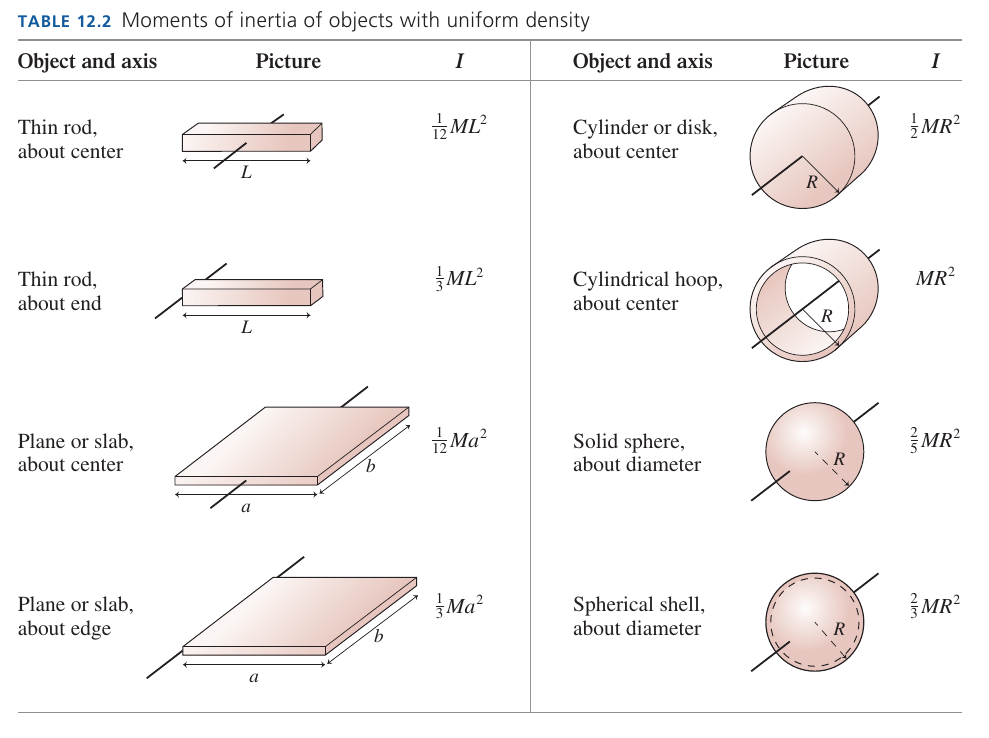
\includegraphics[width=0.7\textwidth]{moment-table.png}

\end{center}



\end{document}
